\documentclass[11pt]{beamer}
\usepackage{hyperref}
\usepackage[T1]{fontenc}
\UseRawInputEncoding

\usepackage{graphicx}
\usepackage[utf8]{inputenc}
\usepackage{mathtools}
\usepackage{verbatim}
\usepackage{smartdiagram}
\usepackage{unicode-math}
%\setmathfont{}
\usepackage{comment}
\usepackage{xcolor}
% Cannot enable in Xelatex
\usepackage{pgfpages}
% \setbeameroption{hide notes} % Only slides
% \setbeameroption{show only notes} % Only notes
% \setbeameroption{show notes on second screen}
\usepackage{latexsym,amsmath,xcolor,multicol,booktabs,calligra}
\usepackage{graphicx,listings,stackengine}

\usepackage{tikz}
\usepackage{tikz-feynman}
\usepackage[compat=1.0.0]{tikz-feynman}
\usepackage{float}

%% Enable only in Xelatex
% \usepackage{pstricks}
\usepackage{feynmp-auto} % or feynmp if you prefer
% Feynman diagrams
%\usepackage{feynmp}
%\usepackage{feynmf}
\DeclareGraphicsRule{*}{mps}{*}{} % for being able to read the produced file

\author{Ana Pereira}
\title{$V_{ud}$ at next-to-next-to-leading order in the electroweak interactions}
\institute [University of Liverpool] {\href{mailto:Ana.Costa-Pereira@liverpool.ac.uk}{\underline{Ana.Costa-Pereira@liverpool.ac.uk}}}
\date{18/06/2025}
\usepackage{QUT}
\usepackage{QUT}

% defs
\def\cmd#1{\texttt{\color{red}\footnotesize $\backslash$#1}}
\def\env#1{\texttt{\color{blue}\footnotesize #1}}
\definecolor{deepblue}{rgb}{0,0,0.5}
\definecolor{deepred}{rgb}{0.6,0,0}
\definecolor{deepgreen}{rgb}{0,0.5,0}
\definecolor{halfgray}{gray}{0.55}

\lstset{
    basicstyle=\ttfamily\small,
    keywordstyle=\bfseries\color{deepblue},
    emphstyle=\ttfamily\color{deepred},    % Custom highlighting style
    stringstyle=\color{deepgreen},
    numbers=left,
    numberstyle=\small\color{halfgray},
    rulesepcolor=\color{red!20!green!20!blue!20},
    frame=shadowbox,
}

\setbeamercolor{block body alerted}{bg=alerted text.fg!10}
\setbeamercolor{block title alerted}{bg=alerted text.fg!20}
\setbeamercolor{block body}{bg=structure!10}
\setbeamercolor{block title}{bg=structure!20}
\setbeamercolor{block body example}{bg=green!10}
\setbeamercolor{block title example}{bg=green!20}

\begin{document}
%
%
% Capa
%
%
\begin{frame}
    \titlepage
    \begin{figure}[htpb]
        \begin{center}
           
\includegraphics[width=0.35\linewidth]{logo.png}
        \end{center}
    \end{figure}
        \begin{figure}[htpb]
        \begin{center}
           
\includegraphics[width=0.35\linewidth]{logo_livinno.jpg}
        \end{center}
    \end{figure}
\end{frame}

\begin{frame}
    \tableofcontents[sectionstyle=show,subsectionstyle=show/shaded/hide,subsubsectionstyle=show/shaded/hide]
\end{frame}

\section{SM and CKM matrix}
\begin{frame}{Standard Model}
    \begin{figure}
        \centering
        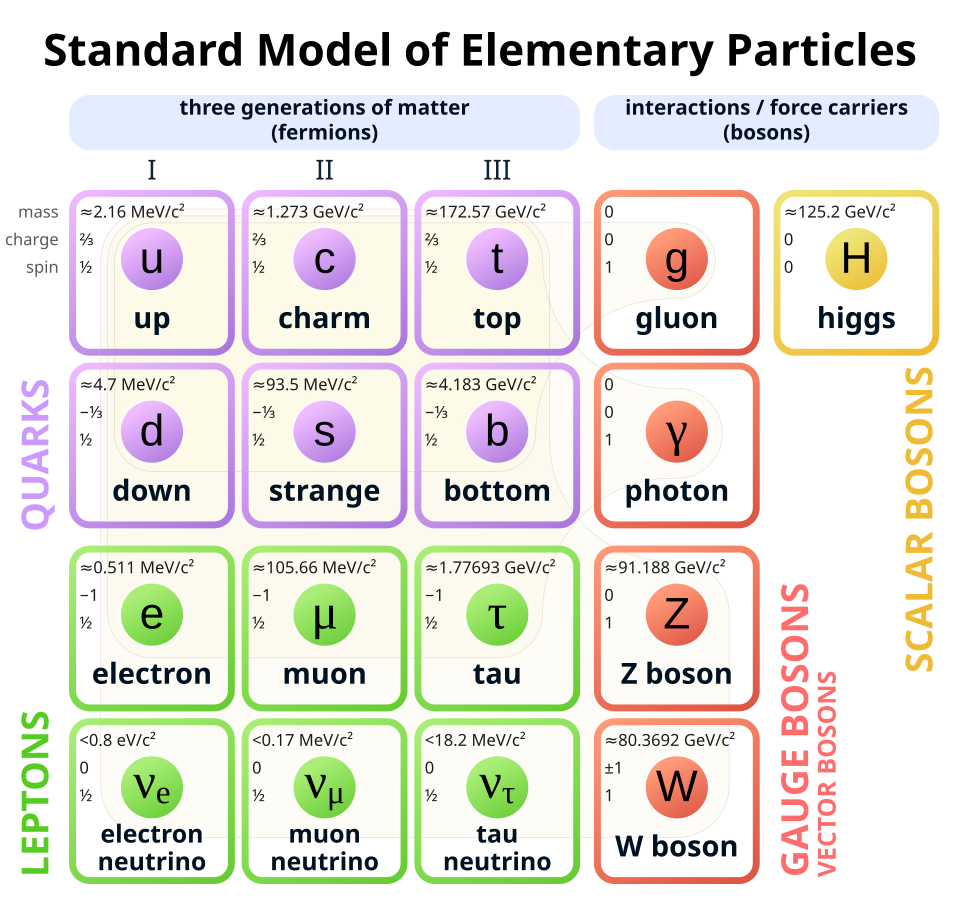
\includegraphics[width=0.6\linewidth]{Standard_Model_of_Elementary_Particles.svg.png}
        \caption{Standard Model}
    \end{figure}
\end{frame}
\begin{comment}
\begin{frame}{Frame Title}
\begin{figure}[H]
\centering
\unitlength = 1.5mm
\begin{fmffile}{V1}
\begin{fmfgraph*}(20,20)
\fmfleft{i1} \fmfright{o1,o2}
\fmflabel{$\psi$}{o2}
\fmflabel{$\Bar{\psi}$}{o1}
\fmflabel{$W$}{i1}
\fmf{photon}{i1,v4}
\fmf{plain_arrow}{o1,v4,o2}
\end{fmfgraph*}
\end{fmffile}
%\caption{Diagram $V_2$}
\begin{fmffile}{V2}
\begin{fmfgraph*}(20,20)
\fmf{plain_arrow}{o1,v4,o2}
\end{fmfgraph*}
\end{fmffile}
\end{figure}
\end{frame}
\end{comment}

\begin{frame}{Weak decays}
\small
    We are interested in charged interactions - mediated by the $W$ bosons.

\begin{figure}
    \centering
    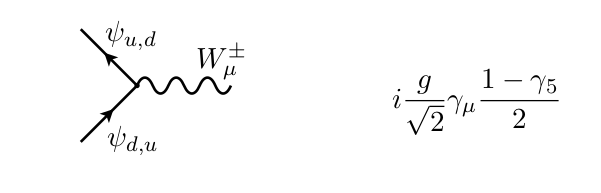
\includegraphics[width=0.6\linewidth]{frule.png}
    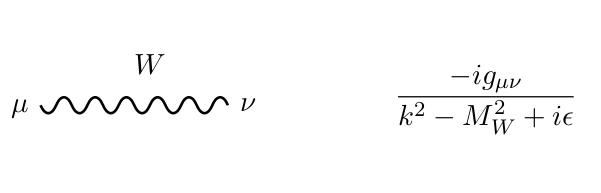
\includegraphics[width=0.6\linewidth]{prop.png}
    \caption{Feynman rules for the Weak Interaction}
\end{figure}

\begin{itemize}
    \item Leptonic decays are decays that involve only leptons and neutrinos;
    \item Semi-leptonic decays are decays that involve quarks and leptons.
\end{itemize}
\end{frame}

\begin{frame}{CKM matrix}
    \begin{figure}
        \centering
        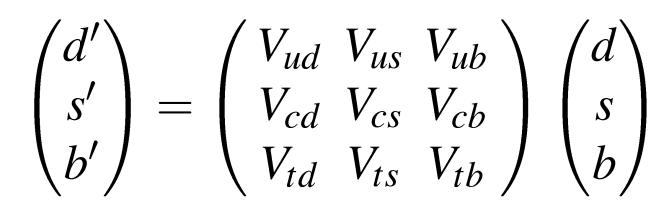
\includegraphics[width=0.5\linewidth]{ckm1.png}
        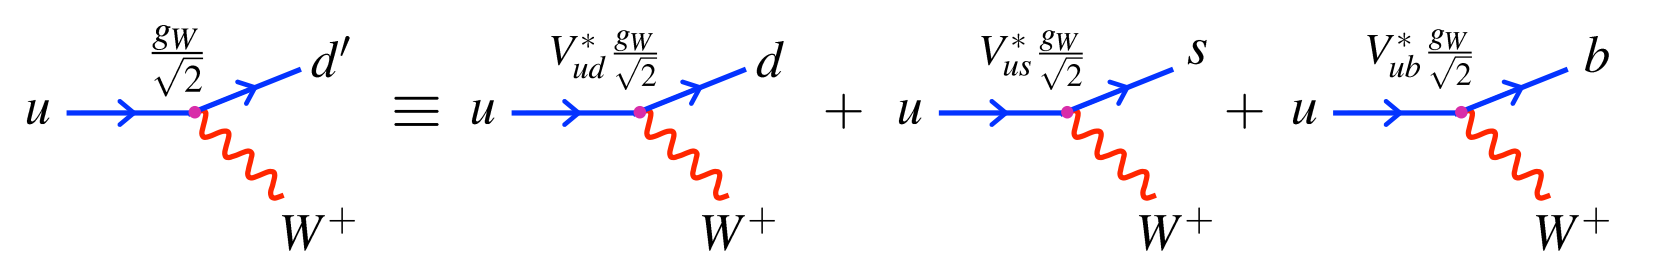
\includegraphics[width=1\linewidth]{ex.png}
        \caption{CKM matrix}
    \end{figure}
    \begin{itemize}
        \item CKM matrix elements are expected complex constants
        \item CKM matrix is expected to be unitary: $V_{CKM}^\dagger V_{CKM} = 1$
    \end{itemize}
\end{frame}

\begin{frame}{CKM Matrix}
The current experimental values for the CKM, from \cite{PDG2024}
\[
\begin{pmatrix}
|V_{ud}| & |V_{us}| & |V_{ub}| \\
|V_{cd}| & |V_{cs}| & |V_{cb}| \\
|V_{td}| & |V_{ts}| & |V_{tb}| 
\end{pmatrix}
=
\]

\[
\begin{pmatrix}
0.97373 \pm 0.00031 & 0.2243 \pm 0.0005 & 0.00394 \pm 0.00036 \\
0.221 \pm 0.004 & 0.987 \pm 0.011 & 0.0422 \pm 0.0008 \\
0.0081 \pm 0.0005 & 0.0394 \pm 0.0023 & 0.9991 \pm 0.0001
\end{pmatrix}
\]

\end{frame}

\begin{frame}{CKM matrix}
The CKM matrix is expected to be unitary in the first row,

\begin{equation}
   \Delta_{CKM} = 1 - |V_{ud}|^2- |V_{us}|^2- O|V_{ub}|^2 =0
\end{equation}
where $|V_{ub}|^2 \approx$  $1.5 \times 10^{-5}$

\begin{figure}
    \centering
    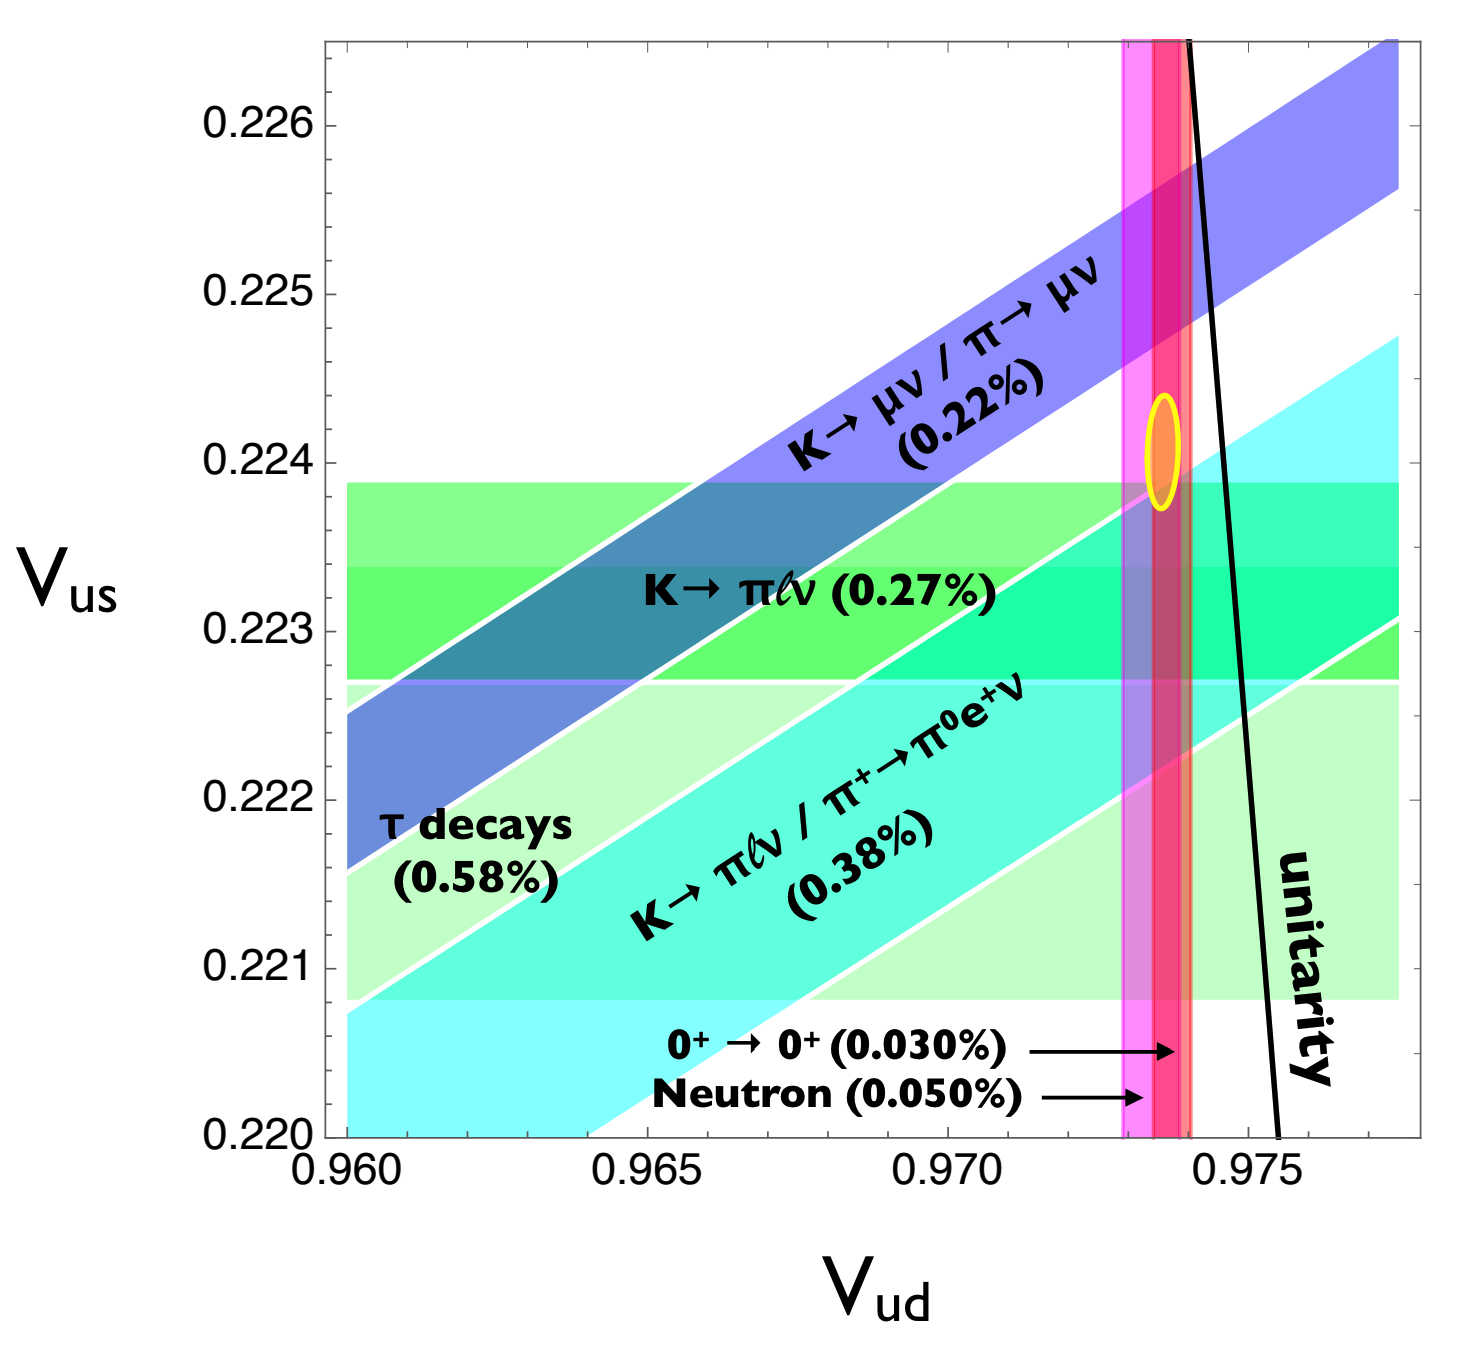
\includegraphics[scale=.2]{ckm.png}
    \caption{\tiny Summary of constraints on $V_{ud}$ and $V_{us}$ (assuming the Standard Model hypothesis) from nuclear, nucleon, meson, and $\tau$ lepton decays., \cite{Bryman:2021teu}.}
\end{figure}

\end{frame}

\begin{frame}{Motivation}
    \begin{itemize}
        \item Compute 2 loop EW corrections relevant for a pion decay;
        \item Match the amplitudes in the full theory to the EFT, to extract the Wilson coefficients (short distance contribution);
        \item WC contribute to later extract the CKM element $V_{ud}$;
        \item Compute the ratio of the pion decay normalized to the muon decay (therefore we compute as well 2 loop EW corrections for the muon decay)
        \item Check that if the pion decay normalized to the muon decay, the only contributions to the WC come from box-type Feynman diagrams.
    \end{itemize}
\end{frame}

\begin{comment}
\begin{frame}{EFT}
What is an \textbf{EFT}?

\begin{itemize}
    \item An EFT is a theoretical framework used to describe phenomena at a specific energy scale without needing to understand all the details of the underlying fundamental theory - it is a low energy approximation
    \item We can obtain an EFT by "integrating out" heavy degrees of freedom (that are only relevant at high energies).
\end{itemize}
\end{frame}
\end{comment}

\section{OPE, Effective Weak Hamiltonian and Wilson coefficients}

\begin{frame}{Tree-level Feynman diagrams in the SM and EFT}
\begin{figure}[H]
\centering

% ---- First Minipage ----
\begin{minipage}[b]{0.45\linewidth}
\centering
\vspace{.2cm}
\resizebox{0.6\linewidth}{!}{ % scale to 90% of minipage width
\begin{fmffile}{eft}
 \begin{fmfgraph*}(120,80)
   \fmfleft{i1,i2}
   \fmfright{o1,o2}
   \fmf{fermion}{i1,v1}
   \fmf{fermion}{i2,v2}
   \fmf{fermion}{v1,o1}
   \fmf{fermion}{v2,o2}
   \fmflabel{$\nu$}{i2}
   \fmflabel{$d$}{i1}
   \fmflabel{$e^{-}$}{o2}
   \fmflabel{$u$}{o1}
   \fmf{photon,label=$W$,label.side=left,label.dist=10}{v1,v2}
 \end{fmfgraph*}
\end{fmffile}
}
\vspace{.2cm}
\caption{SM tree-level.}
\label{treelevelfull}
\end{minipage}
\hfill
\begin{minipage}[b]{0.45\linewidth}
\centering
\vspace{.2cm}
\resizebox{0.6\linewidth}{!}{ % scale to 90% of minipage width
\begin{fmffile}{Full}
 \begin{fmfgraph*}(120,80)
   \fmfleft{i1,i2}
   \fmfright{o1,o2}
   \fmf{fermion}{i1,v1}
   \fmf{fermion}{i2,v1}
   \fmf{fermion}{v1,o1}
   \fmf{fermion}{v1,o2}
   \fmflabel{$\nu$}{i2}
   \fmflabel{$d$}{i1}
   \fmflabel{$e^{-}$}{o2}
   \fmflabel{$u$}{o1}
   \fmfblob{.15w}{v1}
 \end{fmfgraph*}
\end{fmffile}
}
\vspace{.2cm}
\caption{EFT Tree-level.}
\label{treeleveleft}
\end{minipage}
\end{figure}
\small
Evaluating the amplitude $A_{tree}$:

\begin{equation}
    A_{tree} = \frac{- G_F}{2} V_{ud} \frac{g^{\mu \nu}}{k^2 - m_W^2} [\overline{d} \gamma_\mu P_L u ] [\overline{\nu} \gamma_\nu P_L l ] 
\end{equation}

  but if we consider small internal momenta $k << m_W \approx 80 GeV$ we can expand the amplitude. The leading term is given by

    \begin{equation}
    A = \frac{- G_F}{2} V_{ud} \frac{-1}{m_W^2} [\overline{d} \gamma_\mu P_L u ] [\overline{\nu} \gamma_\mu P_L l ] = \frac{- G_F}{2} V_{ud} \frac{-1}{m_W^2} [\overline{d} u ]_{V-A} [\overline{\nu} l ]_{V-A}
\end{equation}
\end{frame}


\begin{frame}{Effective Weak Hamiltonian}
    \textbf{Basic idea of OPE:} the product of two charged current operators is expanded into a series
of local operators, whose contributions are weighted by effective coupling constants, the Wilson coefficients.
    The \textbf{effective weak Hamiltonian} has the following structure

\begin{equation}
    H_{eff}(x) = \dfrac{G_F}{\sqrt{2}} V_{CKM}^{i} C_i(\mu) Q_i(x)
\end{equation}
where
$G_F$ is the \textbf{Fermi constant}
\\
$ V_{CKM}^{i}$ are the \textbf{CKM matrix elements}\\
$C_i$ are the\textbf{ Wilson coefficients} $\longrightarrow$ short distance behavior
\\
$Q_i$ are the \textbf{local operators} $\longrightarrow$ long distance behavior
\end{frame}

\begin{frame}{Physical and Evanescent operators}
\small
    \begin{equation*}
    Q_1 = (\Bar{d} \gamma^{\mu} P_L u ) (\Bar{\nu} \gamma^{\mu} P_L e ) 
\end{equation*}

\begin{equation*}
    Q_1^\mu = (\Bar{\nu_\mu} \gamma^{\mu} P_L \mu  )(\Bar{\nu_e}\gamma^{\mu} P_L e )
\end{equation*}

\begin{equation*}
      E_1 = (\overline{d} \gamma^\mu \gamma^\nu \gamma^\beta P_L u )(\overline{\nu}\gamma_\mu \gamma_\nu \gamma_\beta P_L e)
      - (16- a_q^1 \epsilon)  Q_1
\end{equation*}

\begin{equation*}
      E_1^\mu = (\overline{\nu_\mu} \gamma^\mu \gamma^\nu \gamma^\beta P_L \mu )(\overline{e}\gamma_\mu \gamma_\nu \gamma_\beta P_L e)
      - (16- a^1_\mu \epsilon)  Q_1^\mu
\end{equation*}

\begin{equation*}
      E_2 = (\overline{d} \gamma^\mu \gamma^\nu \gamma^\alpha \gamma^\beta \gamma^\sigma P_L u )(\overline{\nu}\gamma_\mu \gamma_\nu \gamma_\alpha \gamma_\beta \gamma_\sigma P_L e)
      - (256 - a^2_{q} \epsilon )  Q_1 + 20 E_1
\end{equation*}

\begin{equation*}
      E_2^\mu = (\overline{\nu_\mu} \gamma^\mu \gamma^\nu \gamma^\alpha \gamma^\beta \gamma^\sigma P_L \mu)(\overline{\nu_e}\gamma_\mu \gamma_\nu \gamma_\alpha \gamma_\beta \gamma_\sigma P_L e)
      - (256 - a^{2}_{\mu} \epsilon)  Q_1 + 20 E_1
\end{equation*}

\end{frame}

\section{1 loop calculation}
\begin{frame}{1-loop EFT}
\small
The 1-loop EFT diagrams relevant for the pion decay 
\begin{figure}[htbp]
\centering
\begin{minipage}[b]{0.3\linewidth}
\centering
\vspace{.5cm}
\begin{fmffile}{eft1}
 \begin{fmfgraph*}(120,80)
   \fmfleft{i1,i2}
   \fmfright{o1,o2}
    \fmflabel{$\nu$}{i2}
   \fmflabel{$d$}{i1}
   \fmflabel{$e^{-}$}{o2}
   \fmflabel{$u$}{o1}
   \fmf{fermion}{i1,v1,o1}
   \fmf{fermion}{i2,v1,o2}
   \fmffreeze
      \fmf{plain}{i1,v1,v2,o1}
   \fmf{plain}{i2,v1,v3,o2}
      \fmffreeze
\fmf{photon,tension=5,label=$\gamma$,label.dist=10}{v2,v3}
   \fmfblob{.15w}{v1}
 \end{fmfgraph*}
\end{fmffile}
%\caption{Diagram 1}
\end{minipage}
\hfill
\begin{minipage}[b]{0.3\linewidth}
\centering
\vspace{.5cm}
\begin{fmffile}{eft2}
 \begin{fmfgraph*}(120,80)
   \fmfleft{i1,i2}
   \fmfright{o1,o2}
   \fmf{fermion}{i1,v1,o1}
   \fmf{fermion}{i2,v1,o2}
   \fmffreeze
      \fmf{plain}{i1,v2,v1,v3,o1}
      \fmffreeze
\fmf{photon,tension=5,label=$\gamma$,label.dist=10}{v2,v3}
   \fmfblob{.15w}{v1}
 \end{fmfgraph*}
\end{fmffile}
%\caption{Diagram 2}
\end{minipage}
\hfill
\begin{minipage}[b]{0.3\linewidth}
\centering
\vspace{.6cm}
\begin{fmffile}{eft3}
 \begin{fmfgraph*}(120,80)
   \fmfleft{i1,i2}
   \fmfright{o1,o2}
   \fmf{fermion}{i1,v1,o1}
   \fmf{fermion}{i2,v1,o2}
   \fmffreeze
      \fmf{plain}{i1,v2,v1,v3,o2}
      \fmf{plain}{i2,v1,v4,o1}
      \fmffreeze
   \fmf{photon,tension=5}{v2,v4}
   \fmffreeze
\fmf{photon,tension=5,label=$\gamma$,label.dist=10}{v4,v3}
   \fmfblob{.15w}{v1}
 \end{fmfgraph*}
\end{fmffile}
%\caption{Diagram 3}
\end{minipage}
\caption{1-loop EW correction to the EFT theory with radiative corrections. The curved lines represent photons.}
\label{1loopeft}
\end{figure}

Choice of kinematics: external momenta set to zero and all masses bellow the W mass are set to zero. Only masses present in our calculation will be $m_W$, $m_Z$, $m_H$, $m_t$. 
\end{frame}

\begin{frame}{Infrared Rearrangement}

Exact decomposition of a propagator

\begin{equation} \label{IR rearr}
    \dfrac{1}{(k+p)^2-m^2} = \dfrac{1}{k^2-M^2} + \frac{-p^2+ 2 k \cdot p -m^2 + M^2}{k^2-M^2} \frac{1}{(k+p)^2 - m^2}
\end{equation}

 $k$ and $p$ stand for a linear combination of the internal moment and external momenta. The propagator mass is $m$ and $M$ is an introduced fictitious regulator. 
\end{frame}

\begin{frame}{1 loop EFT}
     The sum of the amplitudes of the 1-loop diagrams of the EFT 
\begin{equation}
    M_{EFT} = \int \frac{d^dk}{(4 \pi)^d} \frac{1}{(k^2-M^2)^2}(a_1 Q_1 + a_2 E_1)
\end{equation}

with $a_1$ and $a_2$ being functions dependent on $G_F$, the charges of the particles, the dimension $d$ and the photon gauge $\xi$.
\end{frame}

\begin{frame}{Dimensional Regularisation}
Feynman integral $\longrightarrow$ regularise the divergences $\longrightarrow$ introduce parameter that isolates the divergences 
\\
\vspace{.5cm}
\textbf{DimReg} $\longrightarrow$ space-time dimension is extended to $ 4 \longrightarrow d=4-2\epsilon$. The singularities are the poles when $\epsilon \longrightarrow 0$ 

\begin{equation}
    \textit{2-loop:} \frac{a_1}{\epsilon^2} + \frac{b_1}{\epsilon} + c_1
\end{equation}

with $a_1$, $b_1$ and $c_1$ being constants.\\
\vspace{.1 cm}
The bare EFT amplitude at 1 loop is:
    \begin{equation}
    M_{EFT} = \frac{\alpha}{4 \pi} G_F \frac{1}{\epsilon} (-2 Q_1 - \frac{1}{12} E_1)
\end{equation}
\end{frame}

\begin{frame}{1-loop SM amplitudes}
\centering
    Generate the diagrams with the SM\\
$\downarrow$\\
    Compute the amplitudes $\longrightarrow$ tensor integrals $\longrightarrow$ tensor decomposition $\longrightarrow$ reduction to masters\\
$\downarrow$\\
analytical amplitudes\\
$\downarrow$\\
    $\overline{MS}$ renormalization $\longrightarrow$ renormalized amplitude
\end{frame}

\begin{frame}{1 PI amplitudes in the full SM}
\begin{figure}[h]
\centering
\begin{minipage}[c]{0.45\textwidth}
\begin{tikzpicture}
\begin{feynman}
\vertex (u) at (0,1.5) {\(u\)};
\vertex (a) at (1.5,1.5);
\vertex (d) at (3,1.5) {\(d\)};
\vertex (c1) at (1.5,0.975);
\vertex (c2) at (1.5,0.525);
\vertex (c) at (1.5,0);
\vertex (e) at (0,0) {\(e\)};
\vertex (ve) at (3,0) {\(\nu_e\)};
\diagram* {
  (u) -- [fermion] (a) -- [fermion] (d),
  (a) -- [boson, edge label=\(W\)] (c1),
  (c1) -- [fermion, half left, looseness=1.4, edge label=\(b\)] (c2)
        -- [fermion, half left, looseness=1.4, edge label=\(t\)] (c1),
  (c2) -- [boson, edge label=\(W\)] (c),
  (e) -- [fermion] (c) -- [fermion] (ve),
};
\end{feynman}
\end{tikzpicture}
\end{minipage}
\hfill
\begin{minipage}[c]{0.45\textwidth}
\begin{tikzpicture}
\begin{feynman}
\vertex (u) at (0,1.5) {\(u\)};
\vertex (a) at (1,1.5);
\vertex (a1) at (2,1.5);
\vertex (d) at (3,1.5) {\(d\)};
\vertex (e) at (0,0) {\(e\)};
\vertex (c) at (1,0);
\vertex (c1) at (2,0);
\vertex (ve) at (3,0) {\(\nu_e\)};
\diagram* {
  (u) -- [fermion] (a) -- [fermion, edge label=\(u\)] (a1) -- [fermion] (d),
  (a) -- [boson, edge label'=\(Z\)] (c),
  (a1) -- [boson, edge label=\(W\)] (c1),
  (e) -- [fermion] (c)  -- [fermion, edge label'=\(e\)] (c1) -- [fermion] (ve),
};
\end{feynman}
\end{tikzpicture}
\end{minipage}
%\caption{Some 1 loop diagrams in the full theory for the semi-leptonic decay.}
\label{1loopdiag}
\end{figure}


\begin{figure}[h]
\centering
\begin{minipage}[c]{0.45\textwidth}
\begin{tikzpicture}
\begin{feynman}
\vertex (u) at (0,1.5) {\(u\)};
\vertex (a) at (1,1.5);
\vertex (a1) at (2,1.5);
\vertex (d) at (3,1.5) {\(d\)};
\vertex (e) at (0,0) {\(e\)};
\vertex (c) at (1.5,0);
\vertex (c1) at (1.5,0.6);
\vertex (ve) at (3,0) {\(\nu_e\)};
\diagram* {
  (u) -- [fermion] (a) -- [fermion, edge label=\(d\)] (a1) -- [fermion] (d),
  (a) -- [boson, edge label'=\(W\)] (c1),
  (a1) -- [boson, edge label=\(\gamma\)] (c1),
  (c1) -- [boson, edge label=\(W\)] (c),
  (e) -- [fermion] (c) -- [fermion] (ve),
};
\end{feynman}
\end{tikzpicture}
\end{minipage}
\hfill
\begin{minipage}[c]{0.45\textwidth}
\begin{tikzpicture}
\begin{feynman}
\vertex (u) at (0,1.5) {\(u\)};
\vertex (a) at (1.5,1.5);
\vertex (d) at (3,1.5) {\(d\)};
\vertex (c1) at (1.5,0.75);
\vertex (c2) at (2,0.75);
\vertex (c3) at (2.4,0.75);
\vertex (c) at (1.5,0);
\vertex (e) at (0,0) {\(e\)};
\vertex (ve) at (3,0) {\(\nu_e\)};
\diagram* {
  (u) -- [fermion] (a) -- [fermion] (d),
  (a) -- [boson, edge label'=\(W\)] (c),
  (c1) -- [scalar, edge label=\(H\)] (c2)
        -- [fermion, half left, looseness=1.4] (c3)
        -- [fermion, half left, looseness=1.4, edge label=\(W\)] (c2),
  (e) -- [fermion] (c) -- [fermion] (ve),
};
\end{feynman}
\end{tikzpicture}
\end{minipage}
\caption{Some 1 loop diagrams in the full theory for the semi-leptonic decay.}
\label{1loopdiag}
\end{figure}
\end{frame}


\begin{frame}{Renormalization of the full SM}
The 1 loop counterterms needed are 

\begin{figure}[h]
\begin{minipage}{0.3\textwidth}
% First figure
\begin{tikzpicture}
\begin{feynman}
\diagram[horizontal=a to b] {
  u [particle=\(u\)] -- [fermion] a -- [fermion] d [particle=\(d\)],
  e [particle=\(e\)] -- [fermion] c -- [fermion] ve [particle=\(\nu_e\)],
  a -- [boson, edge label'=\(W\), insertion=0.5, insertion style={cross, very thick}] c,
};
\end{feynman}
\end{tikzpicture}
\end{minipage}
\hfill
\begin{minipage}{0.3\textwidth}
% Second figure
\begin{tikzpicture}
\begin{feynman}
\diagram[horizontal=a to b] {
  u [particle=\(u\)] -- [fermion] a -- [fermion] d [particle=\(d\)],
  e [particle=\(e\)] -- [fermion] c [crossed dot] -- [fermion] ve [particle=\(\nu_e\)],
  a -- [boson, edge label'=\(W\)] c,
};
\end{feynman}
\end{tikzpicture}
\end{minipage}
\hfill
\begin{minipage}{0.3\textwidth}
% Second figure
\begin{tikzpicture}
\begin{feynman}
\diagram[horizontal=a to b] {
  u [particle=\(u\)] -- [fermion] a [crossed dot] -- [fermion] d [particle=\(d\)],
  e [particle=\(e\)] -- [fermion] c -- [fermion] ve [particle=\(\nu_e\)],
  a -- [boson, edge label'=\(W\)] c,
};
\end{feynman}
\end{tikzpicture}
\end{minipage}
\caption{1 loop counterterms in the full theory for the semi-leptonic decay.}
 \label{ctfig}
\end{figure}

In the $\overline{MS}$ scheme we need following renormalization constants

\begin{equation*}
    Z_{M_W}, Z_{M_Z}, Z_{s_W} , Z_{e}, Z_W, Z_u, Z_d, Z_{ele} , Z_\mu, Z_\nu
\end{equation*}
\end{frame}

\begin{frame}{1-loop SM renormalized amplitude}
    Joining all the amplitudes for all type diagrams we obtain the following for the part proportional to the physical operator $Q_1$,
    \small
\begin{equation}
\begin{split}
  & M_{SM} = 
  G_F ( \frac{\alpha}{4 \pi}( a_1 
+ a_2  \ln\left(\frac{m_t^2}{m_W^2} \right)
+ a_3  \ln\left(\frac{M_H^2}{m_W^2} \right)
+ a_4 \ln\left(\frac{M_Z^2}{m_W^2} \right)\\
&
+ a_5 \ln\left(\frac{\mu^2}{m_W^2}  \right) )+ \frac{\alpha}{4 \pi}\frac{(-2)}{\epsilon})
\end{split}
\end{equation}
Notice: we performed renormalization of all physical quantities, but we still have a divergence in the amplitude in the SM.
\vspace{.5cm}
\\
We have the amplitudes now renormalized, so we can do the matching. Let us compute $C_1$ proportional to the physical operator $Q_1$.
\end{frame}

\section{Wilson coefficients}
\begin{frame}{Computation of the Wilson coefficients}
    The Wilson coefficients can be extracting by imposing that the full amplitude (proportional to the physical operator $Q_1$) should match the EFT amplitude (proportional to $Q_1$).

\begin{equation}
    M_{full} = M_{EFT}
\end{equation}

\begin{equation}
\begin{split}
  & C_1 = \frac{\alpha}{4 \pi}( a_1 
+ a_2  \ln\left(\frac{m_t^2}{m_W^2} \right)
+ a_3  \ln\left(\frac{M_H^2}{m_W^2} \right)
+ a_4 \ln\left(\frac{M_Z^2}{m_W^2} \right)\\
&
+ a_5 \ln\left(\frac{\mu^2}{m_W^2}  \right) )
\end{split}
\end{equation}
\end{frame}

\begin{frame}{Wilson Coefficients in the ratio of the decays}
We now do the ratio of 2 effective theories in perturbation theory. The Lagrangian is
\begin{equation}
  \mathcal{L}_{G_F} = -\frac{G_F}{\sqrt{2}} Q_\mu -\frac{G_F}{\sqrt{2}} V_{ud} C_{q} Q_q
\end{equation}

And the Wilson Coefficients are

\begin{align}
  C_{r}^{{LO}}  = 1
\end{align}

\begin{equation}
  C^{NLO}_r = -5 +\frac{a^1_\mu}{4}+\frac{a^1_q}{12} - 2\log\left( \frac{\mu^2}{M_Z^2} \right)\,.
\end{equation}

\begin{itemize}
    \item By analyzing this result we can verify that it comes solely from the box diagrams - all the other topologies cancel.
\end{itemize}
\end{frame}


\section{2 loop calculation}

\begin{frame}{2 loop}
We have generated all the 2 loop order all the box-type diagrams for both the pion and muon decay. The unrenormalised amplitudes were simplified to a final analytical form. 


\begin{figure}[h]
\centering
\begin{tikzpicture}
\begin{feynman}
% Vertices
\vertex (u) at (0,1.5) {\(u\)};
\vertex (a) at (1,1.5);
\vertex (a1) at (2,1.5);
\vertex (a2) at (3,1.5);
\vertex (d) at (4,1.5) {\(d\)};
 
\vertex (e) at (0,0) {\(e\)}; % electron
\vertex (c) at (1,0);         
\vertex (c1) at (2,0);    
\vertex (c2) at (3,0);    
\vertex (ve) at (4,0) {\(\nu_e\)}; % neutrino

\diagram* {
  % Quark line
  (u) -- [fermion] (a) -- [fermion, edge label=\(u\)] (a1) -- [fermion, edge label=\(u\)] (a2) -- [fermion] (d),

  (a) -- [boson, edge label'=\(Z\)] (c),
  (a1) -- [boson, edge label=\(Z\)] (c1),
(a2) -- [boson, edge label=\(W\)] (c2),

  (e) -- [fermion] (c)  -- [fermion, edge label'=\(e\)] (c1)  -- [fermion, edge label'=\(e\)] (c2) -- [fermion] (ve),

};
\end{feynman}
\end{tikzpicture}
\caption{Example of a 2 loop diagram for the pion decay.}
\end{figure}
\end{frame}

\begin{frame}{2 loop counterterms}
    The counterterms at 2 loop were generated to a final analytical form. 

\begin{figure}[h]
\centering
\begin{tikzpicture}
\begin{feynman}
% Vertices
\vertex (u) at (0,1.5) {\(u\)};
\vertex (a) at (1,1.5);
\vertex (a1) at (2,1.5);
\vertex (d) at (3,1.5) {\(d\)};
 
\vertex (e) at (0,0) {\(e\)}; % electron
\vertex (c) at (1,0);         
\vertex (c1) at (2,0);         
\vertex (ve) at (3,0) {\(\nu_e\)}; % neutrino

\diagram* {
  % Quark line
  (u) -- [fermion] (a) -- [fermion, edge label=\(u\)] (a1) -- [fermion] (d),

  (a) -- [boson, edge label'=\(Z\)] (c),
  (a1) -- [boson, edge label=\(W\)] (c1),
  
  (e) -- [fermion] (c)  -- [fermion, edge label'=\(e\)] (c1) -- [fermion] (ve),
};

% Add cross at vertex (c1) = (2,0)
\draw[thick] ($(c1)+(-0.1,0.1)$) -- ($(c1)+(0.1,-0.1)$);
\draw[thick] ($(c1)+(-0.1,-0.1)$) -- ($(c1)+(0.1,0.1)$);

\end{feynman}
\end{tikzpicture}
\caption{Example of counterterms for the 2 loop renormalization}
\end{figure}
\end{frame}

\begin{frame}{2 loop calculation}
\begin{itemize}
    \item We are currently studying the cancellations between diagram types that occurs at 2 loop and generating the 2 loop renormalization constants for external particles.

   \item As our final goal, we aim to compute the 2 loop Wilson coefficients in the pion decay normalized to the muon decay and understand which diagrams contribute to this.
\end{itemize}
\end{frame}

\begin{frame}{Conclusions}
1 loop
    \begin{itemize}
        \item We were able to study how to renormalize the SM and EFT amplitudes to be able to match them
        \item We computed the Wilson coefficients of each decay and checked they were finite
        \item We computed the pion decay normalized to the muon decay, showing that the only contributions that survive com from box-type diagrams
    \end{itemize}
2 loop

\begin{itemize}
    \item We generated the analytical result of the bare amplitudes for the pion and muon decay.
    \item We are generating the 2 loop counterterms and respective renormalization constants
    \item We are working on checking which cancellations occur between diagrams when computed the 2 loop pion decay normalized to the muon decay.
\end{itemize}
\end{frame}

\small
    \bibliographystyle{apalike}
%\printbibliography
\bibliography{slide}
\begin{comment}

\begin{frame}{Physical and Evanescent operator}
        In our case the relevant operators for the pion decay are a physical operator $Q(x)$

\begin{equation}
    Q(x) = (\Bar{d}(x) \gamma^{\mu} P_L u(x) ) (\Bar{\nu}(x) \gamma^{\mu} P_L e(x) ),     \space P_L = \dfrac{1 - \gamma_5}{2}
\end{equation}
\\
and an evanescent operator that can be related with the physical operator

\begin{equation}
E(x) = (\overline{d}(x) \gamma^\mu \gamma^\nu \gamma^\beta P_L u(x)) (\overline{\nu}(x) \gamma_\mu \gamma_\nu \gamma_\beta P_L l(x))
      - (16- a^1_q)  Q(x)
\end{equation}
which vanishes in 4 dimension.
\end{frame}

\begin{frame}{Results for the 1-loop EFT EW corrections for the semi-leptonic decay}
    The sum of the amplitudes $M$ of the 1-loop diagrams of the EFT 
\begin{equation}
    M_{EFT} = \int_k \frac{1}{(k^2-\mu^2)^2}(a_1 Q + a_2 E)
\end{equation}

with 

\begin{equation*}
\begin{split}
   &  a_1 = 
    \frac{\alpha}{4 \pi} G_F \Bigg( Q_u Q_d (\frac{(2-d)^2}{d} - (1 - \xi)) +
     Q_u Q_e (\frac{16}{d} - (1 - \xi))\\
     & + 
     Q_d Q_e (\frac{6d-20}{d} - (1 - \xi)) \Bigg)
\end{split}
\end{equation*}

\begin{equation*}
    a_2 = \frac{\alpha}{4 \pi} \frac{G_F}{d} \Big( Q_u Q_e - Q_d Q_e \Big)
\end{equation*}

with $Q_u$, $Q_d$, $Q_e$ being respectively the quark up, down and electron charges, $\alpha = \frac{e^2}{4 \pi}$ and $\xi$ is the Gauge of the photon.
\end{frame}

\begin{frame}{Infrared Rearrangement}
    The exact decomposition of a propagator which can be done in the following way

\begin{equation} \label{IR rearr}
    \dfrac{1}{(k+p)^2-m^2} = \dfrac{1}{k^2-\mu^2} + \frac{-p^2+ 2 k \cdot p -m^2 + \mu^2}{k^2-\mu^2} \frac{1}{(k+p)^2 - m^2}
\end{equation}

$k$ and $p$ stand for a linear combination of the internal moment and external momenta respectively. The propagator mass is $m$ and $\mu$ is an introduced fictitious regulator for the IR divergences.

\begin{itemize}
    \item Identity can be applied recursively until the overall degree of divergence becomes negative - we can then drop the last term in the decomposition.
    \item  By doing this truncation in the expansion we are making an approximation. The leading divergences will be nevertheless correct since the dropped terms are all UV finite.
\end{itemize}
\end{frame}

\begin{frame}{PV reduction}
\centering
    When generating the amplitudes and simplifying, we will have tensor integrals\\
    $\downarrow$\\
    \textbf{Passarino-Veltman reduction}\\
    $\downarrow$\\
     method of expressing an n-point loop integral with r powers of the loop momentum
l in the numerator, in terms of “scalar” s-point functions\\
\vspace{.5cm}
Tensor integral $\longrightarrow$ Scalar integral $\times$ \{\textbf{metric}, external momenta, levi-civita tensor...\}
\end{frame}
\end{comment}

\end{document}